\chapter{The Paths of Magic}
\label{magic_paths}\index{Magic!Paths of Magic}

\begin{multicols}{2}

There are various roads to learning magic -- each allows the mage to invoke different spheres and has a different flavour of magic.
Any character with the appropriate requirements can learn to cast magic.
Each school of magic has its own flavour but different people casting spells from the same spheres of magic will end up with exactly the same results, mechanically.
A priest of war may call divine fire to to destroy enemies where an alchemist uses precise gestures to summon the essential form of fire, but both are just using the the Invocation sphere.

People can pick up different Paths of Magic by simply fulfilling different requirements. If someone has access to one sphere of magic through multiple Paths and has bought access to the sphere, then learning the same sphere through the different Path simply requires some \gls{downtime} and study but carries no \gls{xp} cost. If a blood sorcerer were to learn the Aldaron sphere as a natural knack and later decided to become an adherent of the goddess Laiqu\"{e}, she could channel the magic through divine means or through her innate abilities.
All that is needed is a little time to pick up an understanding of how this same magic works through a different lens.

\end{multicols}

\section{The Path of Alchemy}\index{Alchemy}

\noindent\textbf{Spheres}: Conjuration, Invocation, Force, Illusion, Metamagic

\begin{multicols}{2}

\noindent The alchemist learns magic through rote repetition and formulae which are usually be invoked through precise hand-gestures and mystical words which are attuned to the background harmonics of the universe.  Alchemy was invented by the gnomes but has since become popular with various upper-class humans. This is the typical magic of a standard town wizard. Alchemy requires one slot of Academics in order to be learnt.

Spells summoned by the Path of Alchemy are accompanied by magical sparks and sometimes loud bangs. Their mana stones are always based on precious minerals or rocks such as rubies, sapphire or even diamonds. 

\subsection{Special Considerations}

Without the ability to move one's hands and use one's voice, alchemy spells take a -2 penalty to any task roll or a -4 penalty if the mage can neither move nor use their voice.

Alchemists cannot naturally intuit how the next level of any sphere works.
Instead they must pick up levels slowly and through intense study.
They only receive new levels during \gls{downtime}.

\subsection{Mana Stones}

Alchemical mana stones are always precious items, such as gold, rubies, or diamonds.  A mana stone costs 10 gp per \gls{mp} which can be stored inside it, so a mana stone storing 3 \gls{mp} would cost 30 gp. The exact item might be a simply ruby which stores mana, a diamond-headed wand of ivory which blasts out fireballs or a sword with jewels on the handle which surrounds the warrior with moving illusions of their. Alchemical mana stones with a spell always activate those spells with a command word.

\end{multicols}

\section{The Path of Blood}

\textbf{Spheres}: Aldaron, Enchantment, Force, Invocation, Polymorph

\begin{multicols}{2}

\noindent Certain races, such as elves and dragons, are naturally magical and can learn forms of innate magic. Some humans with a touch of elven (or even draconic) blood have been known to walk the Path of Blood.

Blood magic spells cast quickly appear in a flurry of inky darkness, meanwhile the caster's eyes glow red and lightning flashes around their head.

Blood sorcerers need only use movements to cast their spells. Without the ability to move freely they suffer a -2 penalty to casting spells.

\subsection{Special Considerations}

Most elves look down upon people who learn magic through rote facts and dusty tomes, seeing their innate connection to the magic of the world as a higher and purer form of magical ability.

Blood sorcerers are barred from ritual castings -- spending all day trying to cast a spell will not help in the slightest. They cannot cast subtle spells, so enchantment effects will always be at least a little noticeable to those watching out for them, at least at the time of casting.

Blood magic casters who learn Metamagic through another path of magic cannot use Metamagic spells to modify spheres they only have through blood magic.
For example if an elf learnt how to cast Metamagic through the path of song, they couldn't use that Metamagic sphere to modify their Invocation spells if they only learnt Invocation through the Path of Blood.

\end{multicols}

\section{The Path of Devotion}

\textbf{Spheres}: Aldaron, Fate, Metamagic and two from the deity's schools of choice.

\begin{multicols}{2}

\noindent The character is devoted to a god and studies with priests in how to unlock the magic of the deity. The character's god will determine their additional spheres of magic and their appearance.

One slot of Academics is required to be able to sufficiently understand the precepts of the deity and the elaborate prayers. Specifically, characters must specialise in Theology. Devoting oneself to multiple deities is possible, so long as those deities are not antagonistic to each other, however, each deity requires an additional Theology specialisation. The appearance of spells and the form of mana stones varies depending upon deity.

This path is most commonly taken by humans and the occasional gnoll. Gnomes don't acknowledge gods, elves think they \emph{are} gods and dwarves tend to view their own rune magic as divine in a very general sense.

\subsection{Special Considerations}

The path of devotion requires casters to both use their voice and to move their hands, as per Alchemy. Failure to do either one results in a -2 penalty. So using one's hands to wield a weapon while being underwater would give a -4 penalty to any spells cast.

\subsection{Mana Stone}

Each type of devotion has its own mana stone.  See the individual references on page \pageref{gods_codes}.

\end{multicols}

\section{The Path of Runes}

\index{Runes}\textbf{Spheres}: Conjuration, Fate, Force, Metamagic, Necromancy

\begin{multicols}{2}

\noindent Dwarves are skilled in the art of summoning magics through carving elaborate runes. Typically they are chiselled, but it is possible to simply `paint a spell' onto a surface.

When spells are summoned, the runes glow -- whether carved or painted -- then giant, ghostly runes can be seen dancing around the source of the spell.
Runecrafters summoning acid rain might have their spell appear with a flurry of glowing symbols of trickery -- each sphere of magic and indeed each spell has its own special runes.

Runecasters must devote a single Academics slot to learning how to properly inscribe runes. Their mana stones are always precious metals inscribed with runes such as armour with platinum runes or swords with golden runic inlays. Those mana stones which have an imprinted spell can be activated by either a command word or a condition.

\subsection{Special Considerations}

Runecasters cannot cast spells in the heat of combat -- inscribing runes just takes far too long for Quick Spells. They always use Ritual Spells for the highest level of any Sphere, and can use normal casting after that.

However, in return for this deficite, runecasters can learn their craft far more easily. Each level of a sphere they purchase costs 5 \gls{xp} less than it normally would. While buying Fate 2 would normally cost 10 for the first level and 15 for the second, runecasters merely need to spend 5 \gls{xp} for the first level and 10 for the second. If they ever want to use those same sphere through a different path of magic, they must spend 5 \gls{xp} to `repurchase' each level. For example, someone who could cast both alchemical and runic magic might purchase Conjuration at the second level for a total of 15 \gls{xp}. They could only use it for runic magics, but later they could spend 5 \gls{xp} to be able to cast the first level with either the alchemy path or the runecasting path.

Runes can never be cast in a subtle way. All castings will be entirely obvious. Ritual castings are a particularly long affair, often taking an entire day's work and always require runes to be dented or impressed into something rather than just written out.

\subsection{Mana Stones}

Rune casters mana stones are, of course, runic carvings, and can never be painted onto anything.

\iftoggle{verbose}{
	\noindent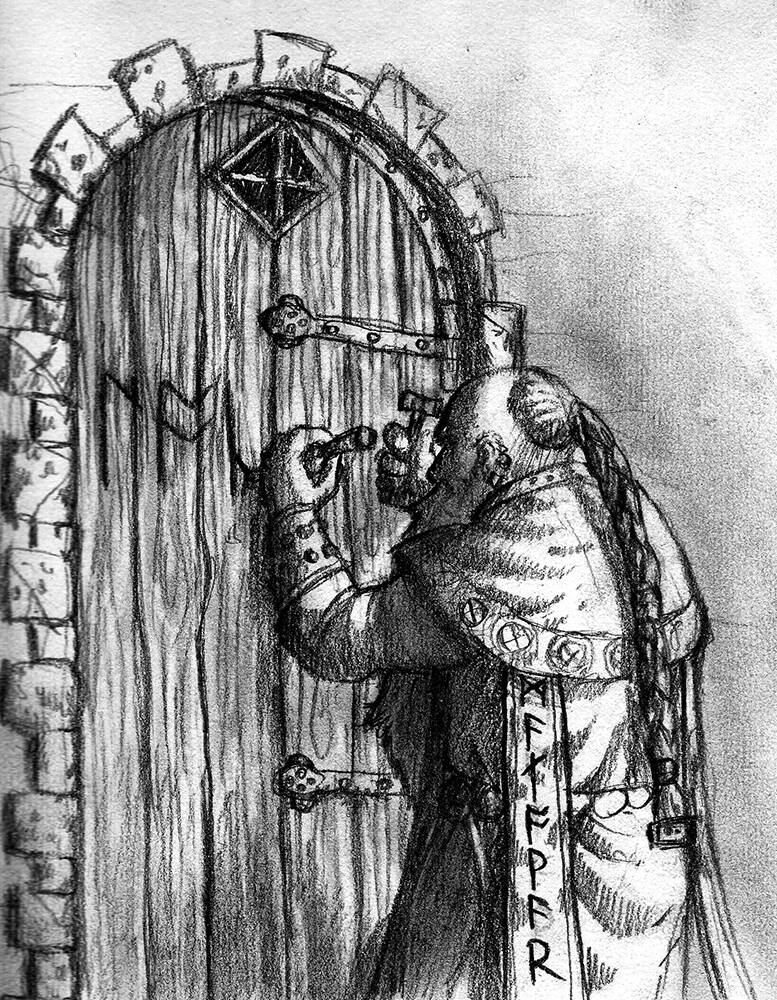
\includegraphics[width=\linewidth]{images/Roch_Hercka/dwarvish_runes.jpg}
	\label{roch:runes}
}{}

\end{multicols}

\section{The Path of Song}

\label{song}\textbf{Spheres}: Aldaron, Enchantment, Fate, Illusion, Metamagic

\begin{multicols}{2}

The character has learnt the magic of song. They can sing illusions into existence, inspire people with great tales and enchant people with a lute. Any instrument, song or performance suffices for casting a spell so long as it is appropriate -- a flute is not usually a good way to magically make people scared.

Song spells appear with a flash of colour -- generally on a cinematically appropriate note. They require some noise to activate so they are difficult to hide, but people will not always make the connection between the start of a spell and the strumming of a lyre.

In order to learn the Path of Song, the mage must have the second level of the Performance Skill. 

\subsection{Special Considerations}

Just as with rune magic, song magic can never be cast in an instant.  Their highest level of a sphere can only be cast as a ritual spell, and quick spells are entirely barred, as a song takes time to be invoked with magic.  And as with rune magic, those on this Path need to spend 5 less \gls{xp} each time they buy a level of some magic sphere.

\subsection{Mana Stones}

The mana stones of the Path of Song are actual songs. The bard composes a song especially for the purpose; when anyone -- anywhere in the world -- plays the song on the correct instrument the mana can be regained. Such songs can also become vessels for spells, becoming magical items which activate once played.

If anyone ever pulls mana from the song (either for a spell casting or because they are low on mana) while the song-spell is empty, it is destroyed forever. The song will be difficult for anyone to remember and will no longer store any mana until someone remakes the spell.

Rare and powerful spell-songs are swapped as currency among bards -- spells which can protect the singer or enchant a crowd.

\end{multicols}


